% -*- mode: LaTeX; coding: utf8; -*-
\documentclass[a4paper,12pt]{extreport}
\usepackage[utf8]{inputenc} 
\usepackage[T2A]{fontenc}
\usepackage[ukrainian]{babel}
\usepackage{pgfplots}
\usepackage{indentfirst} 
\usepackage[pdftex,unicode,bookmarks]{hyperref}
\usepackage[section]{placeins}
\usepackage{amsmath}  
\usepackage{amsfonts}
\usepackage{color}
\definecolor{bluegray}{RGB}{230,230,255}
\usepackage{listings}
% \lstset{
%     extendedchars=\true, 
%     inputencoding=utf8,
%     breaklines=true,
%     basicstyle=\ttfamily, 
%     numbers=left,
%     frame=single,
%     backgroundcolor=\color{bluegray}
% }
% \lstset{language=Python}
% \lstset{frame=lines}
% \lstset{caption={Insert code directly in your document}}
% \lstset{label={lst:code_direct}}
% \lstset{basicstyle=\footnotesize}
\usepackage{pythonhighlight}
\usepackage{verbatim}
\usepackage{setspace} 
\onehalfspacing
\usepackage{geometry}  % поля
\geometry{a4paper}
\geometry{left=15mm,right=15mm,top=20mm,bottom=20mm}
\geometry{headheight=2ex,headsep=10mm,footskip=10mm}
\newtheorem{theorem}{Теорема}[section]
\newtheorem{corollary}{Означення}[theorem]
\newtheorem{lemma}[theorem]{Lemma}
\usepackage{graphicx} %для картинок
\usepackage{caption}
\usepackage{algorithm} 
\usepackage{algpseudocode}
\begin{document}
    \begin{titlepage}%
        \begin{center}
            {ЛЬВІВСЬКИЙ НАЦІОНАЛЬНИЙ УНІВЕРСИТЕТ \\ ІМЕНІ ІВАНА ФРАНКА}\par
            {МЕХАНІКО-МАТЕМАТИЧНИЙ ФАКУЛЬТЕТ \\ КАФЕДРА МАТЕМАТИЧНОЇ ЕКОНОМІКИ ТА ЕКОНОМЕТРИКИ}\par
            \begin{center}
            
\includegraphics[height=4cm]{figures/title_mexmat.jpg}
            \end{center}
            \vspace{10mm}
            \bf{\small{МАГІСТЕРСЬКА КВАЛІФІКАЦІЙНА РОБОТА}}\par
        {\small{на тему:}}\par
            \vspace{20mm}
            {\LARGE{\bf{\scshape{Оптимальне керування системою реакції дифузії та його чисельна реалізація}}}}\par
            \vspace{5mm}
            {}\par %subtitle
        \end{center}
        \vfill
        \hfill
        \begin{flushright}
        \begin{minipage}[t]{80mm}
            \flushright
            студента VI курсу\\
            групи МТЕМ-21\\
            {Войтовича Ярослава}\par
            \vspace{2ex}
            Науковий керівник:\\
            {доцент}\\
            Флюд В. М.
        \end{minipage}
        \end{flushright}
        
        \begin{center}Львів --- 2022\end{center}
    \end{titlepage}
    \stepcounter{page}
\tableofcontents
\newpage 
\chapter{Вступ} 
Моделювання динамічних систем лежить в основі багатьох галузей людської життєдіяльності, 
які мають справу зі змінними в часі процесами. Традиційно можна виділити три задачі такого моделювання, а 
саме описову, предиктивну та прескриптивну. Рішення описових задач зазвичай полягає у відповіді на запитання 
про поточний або минулий стан розглянутої моделі, тоді як предиктивні задачі потребують пошуку можливих станів 
системи у майбутньому. Прескриптивні задачі включають більш глибокий аналіз системи в тому сенсі, що не лише вимагають
відповіді на запитання про майбутній стан системи, а також встановлення множини рішень, що допоможуть досягнути 
деяких бажаних станів відповідно до контексту задачі. Задачі оптимального керування є підмножиної 
таких прескриптивних задач математичного моделювання. Метою задач оптимального керування є пошук контролю 
динамічної системи, при якому деяка задана цільова функція набуває оптимального значення.
Розвитку набули підходи оптимального керування як для детермінованих так і для стохастичних динамічних систем, з неперервними 
та дискретними значеннями часу. 
Значна частина підходів базується на методах варіаційного числення, методах динамічного програмування, описаних Річардом Беллманом, та 
принципі максимуму Понтрягіна.

У цій роботі розглядається оптимальне керування виключно детермінованими процесами та чисельні методи з принципом Понтрягіна [] в їх основі.

\section{Постановка задачі} 
Розглянемо задачу оптимального керування, що визначається цільовою функцією, та деякою динамічною системою, яка змінюється з часом і залежить від
керування. Динамічна система визначається заданою ситсемою диференційних рівнянь. Якщо задача є коректною для використання 
принципу максимуму Понтрягіна, можна
встановити систему з необхідних умов для максимізації функціоналу та визначити
множину в просторі допустимих керувань, що дозволяє знайти оптимальний розв'язок. 
Відносно прості системи дозволяють знайти розв'язок аналітично, проте в загальному випадку системи з багатьох рівнянь 
з розмірністю змінної простору понад дві координати часто необхідно використати чисельні апроксимації для знаходження 
розв'язку. Реалізації алгоритмів для пошуку оптимального керування є актуальними на сьогодні. Існує велика кількість програмних
пакетів та бібліотек, що на різних рівнях абстракції пропонують рішення задач оптимального керування. Основною проблемою 
створення універсального інструмента є індивідуальні підходи для вирішення кожного класу задач оптимального керування.  
Часто для розвязку подібних задач достатньо поєднати методи з пакетів лінійного та нелінійного програмування, а також чисельної 
апроксамиції диференційних систем методи скінченних різниць, скінченних елементів або скінченних об'ємів. Так компанія-розробник 
популярного середовища MathWorks не пропонує окремого пакета для написання рішень оптимального керування, але надає ряд статей 
та рекомендацій по розробці подібних програм з використанням вже існуючих пакетів \cite{1}, \cite{2}. 
\chapter{Основна частина} 
\section{Визначення принципу Понтрягіна} 
Введемо формальне означення задачі оптимального керування для динамічної системи в загальному вигляді. 
    %\subsubsection*{Означення 2.1.1}
    \begin{corollary}
    Максимізувати функціонал
    \begin{equation} \label{eq:2_1}
      \mathcal{L}\left(u, x^u\right)=\int_0^T G\left(t, u(t), x^u(t)\right) d t+\varphi\left(x^u(T)\right)
    \end{equation}   
    \newline по
    $u \in K \subset L^2\left(0, T ; \mathbb{R}^m\right)(T>0)$, де  $x^u$ є розв'язком наступної системи, що називається рівнянням стану системи
    \begin{equation} \label{eq:2_2}
        \left\{\begin{array}{l}
        x^{\prime}(t)=f(t, u(t), x(t)), \quad t \in(0, T) \\
        x(0)=x_0
        \end{array}\right.
    \end{equation}
    Для задачі на мінімум можна переформулювати задачу наступним чином:
    $$ \text{Мінімізувати}  \left\{-\mathcal{L}\left(u, x^u\right)\right\}
    \text { відносно } u \in K \subset L^2\left(0, T ; \mathbb{R}^m\right)$$
    \end{corollary} 
Введемо означення принципу максимуму Понтрягіна. Для цього задамо необхідні умови для функцій задачі оптимального керування.
Нехай функції задачі задовольняють наступні умови:
    $$
    \begin{aligned}
    &G:[0, T] \times \mathbb{R}^m \times \mathbb{R}^N \rightarrow \mathbb{R} \\
    &\varphi: \mathbb{R}^N \rightarrow \mathbb{R} \\
    &f:[0, T] \times \mathbb{R}^m \times \mathbb{R}^N \rightarrow \mathbb{R}^N
    \end{aligned}
    $$
$$
    x_0 \in \mathbb{R}^N, m, N \in \mathbb{N}^*, \text { and } K \subset L^2\left(0, T ; \mathbb{R}^m\right)
$$
    Назвемо $u^* \in K$ назвемо  оптимальним розв'язком задачі оптимального контролю, якщо
    $\mathcal{L}\left(u^*, x^{u^*}\right) \geq \mathcal{L}\left(u, x^u\right),$
    для усіх $u \in K$. Пара $\left(u^*, x^{u^*}\right)$ називається оптимальною парою і $\mathcal{L}\left(u^*, x^{u^*}\right)$ називається оптимальним значенням функції вартості. Ми також називаємо $\left(u^*, x^*\right)$ оптимальною парою якщо $u^*$ є оптимальним керуванням і $x^*=x^{u^*}$.
    Нехай $u^* \in K$ є оптимальним задачі оптимального керування, тоді:
    \begin{equation} \label{eq:2_3}
        \int_0^T G\left(t, u^*(t), x^{u^*}(t)\right) d t+\varphi\left(x^{u^*}(T)\right) \geq \int_0^T G\left(t, u(t), x^u(t)\right) d t+\varphi\left(x^u(T)\right)
    \end{equation}
    для усіх $u \in K$.
    Далі вважатимемо, що для функцій задачі виконуються наступні умови:
    $$
        \left\{\begin{array}{l}
            f_u=\frac{\partial f}{\partial u}, \quad f_x=\frac{\partial f}{\partial x} \\
            G_u=\frac{\partial G}{\partial u}, \quad G_x=\frac{\partial G}{\partial x} \\
            \varphi_x=\frac{\partial \varphi}{\partial x}
        \end{array}\right.
    $$
    % Формулювання принципу Понтрягіна
    Розглянемо множину V.
    $$
        V=\left\{v \in L^2\left(0, T ; \mathbb{R}^m\right) ; u^*+\varepsilon v \in K \text { для усіх достатньо малих } \varepsilon>0 \right\}
    $$
    Введемо функцію $z$ як диференціал від $x$ по $v$: $z=d x^{u^*}(v)$. 
    Оскільки за визначенням повного диференціалу:
    $$ d z=z_x^{\prime} d x+z_y^{\prime} d y $$
    функція $z$ є розв'язком наступної системи:
    \begin{equation} \label{eq:2_4}
        \left\{\begin{array}{l}
            z^{\prime}(t)=f_u\left(t, u^*(t), x^{u^*}(t)\right) v(t)+f_x\left(t, u^*(t), x^{u^*}(t)\right) z(t), \quad t \in(0, T) \\
            z(0)=0
        \end{array}\right.
    \end{equation}
    З умови оптимальності \ref{eq:2_3} випливає нерівність:
    \begin{equation} \label{eq:2_5}
        \begin{aligned}
            \int_0^T G\left(t, u^*(t), x^{u^*}(t)\right) d t+\varphi\left(x^{u^*}(T)\right) \geq & \int_0^T G\left(t, u^*(t)+\varepsilon v(t), x^{u^*+\varepsilon v}(t)\right) d t \\
            +\varphi\left(x^{u^*+\varepsilon v}(T)\right),
        \end{aligned}
    \end{equation}
    Перегрупуємо нерівність \ref{eq:2_5} та поділом на $\varepsilon$:
    $$
    \begin{aligned}
    &\int_0^T \frac{1}{\varepsilon}\left[G\left(t, u^*(t)+\varepsilon v(t), x^{u^*+\varepsilon v}(t)\right)-G\left(t, u^*(t), x^{u^*}(t)\right)\right] d t \\
    &+\frac{1}{\varepsilon}\left[\varphi\left(x^{u^*+\varepsilon v}(T)\right)-\varphi\left(x^{u^*}(T)\right)\right] \leq 0
    \end{aligned}
    $$
    Оскільки можемо обирати $\varepsilon$ як завгодно малим, то перейдемо до диференціалів. Формула повного диференціала функції G:
    $$
    d G=G_u^{\prime} d u+G_x^{\prime} d x
    $$
    Враховуючи значення диференціалів описані вище, перейдемо до настпупного вигляду:

    $$
    \begin{aligned}
    &\int_0^T\left[v(t) \cdot G_u\left(t, u^*(t), x^{u^*}(t)\right)+z(t) \cdot G_x\left(t, u^*(t), x^{u^*}(t)\right)\right] d t \\
    &+z(T) \cdot \varphi_x\left(x^{u^*}(T)\right) \leq 0
    \end{aligned}
    $$
    Далі розглянемо так звану спряжену проблему. p - це спряжений стан. Це необхідна умова першого порядку у визначенні принципу Понтрягіна.
    \begin{equation} \label{eq:2_6}
    \left\{\begin{array}{l}
    p^{\prime}(t)=-f_x^*\left(t, u^*(t), x^{u^*}(t)\right) p(t)-G_x\left(t, u^*(t), x^{u^*}(t)\right), \quad t \in(0, T) \\
    p(T)=\varphi_x\left(x^{u^*}(T)\right)
    \end{array}\right.
    \end{equation}
    Якщо помножити рівняння \ref{eq:2_4} на $p$ та проінтегрувати частинами, то отримаємо рівність:
    $$
    \begin{aligned}
    &z(T) \cdot p(T)-\int_0^T z(t) \cdot p^{\prime}(t) d t \\
    &=\int_0^T\left[f_u\left(t, u^*(t), x^{u^*}(t)\right) v(t)+f_x\left(t, u^*(t), x^{u^*}(t)\right) z(t)\right] \cdot p(t) d t
    \end{aligned}
    $$
    Далі підставляємо p, за визначенням зі спряженої задачі:
    \begin{equation} \label{eq:2_7}
    \begin{aligned}
    &z(T) \cdot \varphi_x\left(x^{u^*}(T)\right) \\
    &+\int_0^T z(t) \cdot\left[f_x^*\left(t, u^*(t), x^{u^*}(t)\right) p(t)+G_x\left(t, u^*(t), x^{u^*}(t)\right)\right] d t \\
    &=\int_0^T\left[v(t) \cdot f_u^*\left(t, u^*(t), x^{u^*}(t)\right) p(t)+z(t) \cdot f_x^*\left(t, u^*(t), x^{u^*}(t)\right) p(t)\right] d t
    \end{aligned}
\end{equation}
    Можна звести \ref{eq:2_7} до вигляду:
    $$
    \begin{aligned}
    &\int_0^T z(t) \cdot G_x\left(t, u^*(t), x^{u^*}(t)\right) d t+z(T) \cdot \varphi_x\left(x^{u^*}(T)\right) \\
    &=\int_0^T v(t) \cdot f_u^*\left(t, u^*(t), x^{u^*}(t)\right) p(t) d t
    \end{aligned}
    $$
    $$
    \int_0^T v(t) \cdot\left[G_u\left(t, u^*(t), x^{u^*}(t)\right)+f_u^*\left(t, u^*(t), x^{u^*}(t)\right) p(t)\right] d t \leq 0
    $$
    $$
    G_u\left(\cdot, u^*, x^{u^*}\right)+f_u^*\left(\cdot, u^*, x^{u^*}\right) p \in N_K\left(u^*\right)
    $$
    Це також необхідна умова першого порядку у визначенні принципу Понтрягіна.
    Ця множина є нормальним конусом.
    Далі розглянемо схему доведення існування оптимального за Понтрягіним контролю.
    Також визначимо принцип Понтрягіна через гамільтоніан 
    Умови трансверсальності для принципу максимуму Понтрягіна 
\subsection{Схема довдення існування оптимального керування}
Нехай 
$$
d=\sup _{u \in K} \mathcal{L}\left(u, x^u\right) \in \mathbb{R} .
$$
Для усіх $n \in \mathbb{N}^*$ , існує $u_n \in K$ такий, що:
$$
d-\frac{1}{n}<\mathcal{L}\left(u_n, x^{u_n}\right) \leq d
$$
Крок 1. Довести, що існує підпослідовність $\left\{u_{n_k}\right\}$, така що:
$$
u_{n_k} \longrightarrow u^* \text { слабко збігається в } L^2\left(0, T ; \mathbb{R}^m\right)
$$
Крок 2. Довести, що існує підпослідовність $\left\{x^{u_{n_r}}\right\}$ послідовності $\left\{x^{u_{n_k}}\right\}$, що збігається до $x^{u^*}$ на $C\left([0, T] ; I R^N\right)$.
Крок 3. 
З нерівності:
$$
d-\frac{1}{n_r}<\mathcal{L}\left(u_{n_r}, x^{u_{n_r}}\right) \leq d
$$
Переходимо границі і отрмаємо:
$$
\mathcal{L}\left(u^*, x^{u^*}\right)=d
$$
$u^*$ - оптимальне керування задачі.
\section{Градієнтний метод для оптмального керування} 
Розглянемо задачу оптимального керування:
\begin{equation} \label{eq:3_1}
\text { Максимізувати } \Phi(u)=\mathcal{L}\left(u, x^u\right)=\int_0^T G\left(t, u(t), x^u(t)\right) d t
\end{equation}
відносно $u \in K \subset U=L^2\left(0, T ; \mathbb{R}^m\right)(T>0)$, де $x^u$ є розв'язком рівняння стану:
\begin{equation} \label{eq:3_2}
\left\{\begin{array}{l}
x^{\prime}(t)=f(t, u(t), x(t)), \quad t \in(0, T) \\
x(0)=x_0
\end{array}\right.
\end{equation}
    Переформулюємо як задачу пошуку мінімуму:
$$
    \text{Мінімізувати } \Psi(u)=-\mathcal{L}\left(u, x^u\right)
$$
$$
    \Psi(u)=-\Phi(u)
$$
    Використаємо метод проекції градієнта для пошуку мінімуму.
    \newline
    Крок 1. Обираємо довільний вектор керування $u^{(0)} \in K$, присвоюємо $k:=0$.
    \newline
    Крок 2. Шукаємо розвязок $x^{(k)}$ з рівняння стану:
$$
    \left\{\begin{array}{l}
        x^{\prime}(t)=f\left(t, u^{(k)}(t), x(t)\right), \quad t \in(0, T) \\
        x(0)=x_0
    \end{array}\right.
$$
\newline
    Крок 3. Шукаємо спряжений стан $p^{(k)}$ зі спряженої системи:
$$
    \left\{\begin{array}{l}
        p^{\prime}(t)=-f_x^*\left(t, u^{(k)}(t), x^{(k)}(t)\right) p(t)-G_x\left(t, u^{(k)}(t), x^{(k)}(t)\right), \quad t \in(0, T) \\
        p(T)=0 .
    \end{array}\right.
$$
\newline
    Крок 4. Обчислюємо градієнт функції втрат:
$$
    w^{(k)}:=\Phi_u\left(u^{(k)}\right)=G_u\left(\cdot, u^{(k)}, x^{(k)}\right)+f_u^*\left(\cdot, u^{(k)}, x^{(k)}\right) p^{(k)} .
$$
\newline
    Крок 5. Визначаємо розмір кроку градієнтного спуску $\rho_k \geq 0$:
$$
    \Phi\left(P_K\left(u^{(k)}+\rho_k w^{(k)}\right)\right)=\max _{\rho \geq 0} \Phi\left(P_K\left(u^{(k)}+\rho w^{(k)}\right)\right)
$$
\newline
Крок 6. 
$$
    u^{(k+1)}:=P_K\left(u^{(k)}+\rho_k w^{(k)}\right)
$$
Критерії зупинки.
$$
    \text { Якщо }\left\|u^{(k+1)}-u^{(k)}\right\|<\varepsilon
$$
$u^{(k+1)} \text { є шуканаю апроксимацією оптимального керування }$. В іншому разі виконуємо присвоєння $k:=k+1$ і повертаємось до кроку 2.

$P_K$ - оператор проекції градієнта на опуклу множину $K$.  Метод проекції градієнта враховує можливість додаткових обмежень на множині допустимого оптимального керування $U$. $$
P_K: U \rightarrow K
$$
    Якщо оптимальне керування не є обмеженим на $U$,  то крок 5 набуває вигляду:
$$
    \Phi\left(u^{(k)}+\rho_k w^{(k)}\right)=\max _{\rho \geq 0}\left\{\Phi\left(u^{(k)}+\rho w^{(k)}\right)\right\}
$$
Алгоритм у форматі псевдокоду приведений нижче:
\begin{algorithm}[H]
	\caption*{Метод Арміджіо} 
	\begin{algorithmic}[1]
		\While{Евклідова норма вектора градієнта строго перевищує $\varepsilon$ або крок градієнта строго перевищує $ \rho_j$}
            \State Розв'язати рівняння стану відповідно до поточних значень функції керування $currentU$;
            \State Розв'язати рівняння стану відповідно до поточних значень функції керування $currentU$ та стану $x$;
            \State Обчислити градієнт функції втрат з урахуванням обчислених функцій $currentU$, $x$ та $p$;
            \If {Евклідова норма градієнта менша $\varepsilon$}
                \State break
            \EndIf
            \State Встановити початкове значення кроку градієнта $currentGradientStep=initGradientStep$;
			\For {$gradientIteration=1,2,\ldots,MaxGradientIteration$}
                \State Оновити функцію керування $ newU = prevU - currentGradientStep * currentGradient $
                \State Розв'язати рівняння стану відповідно до поточних значень функції керування $newU$;
                \State Розв'язати рівняння стану відповідно до поточних значень функції керування $newU$ та стану $x$;
                \State Обчислити значення функції втрат $ newCost $
                \If {$ newCost >= prevCost $}
                    \State Поправка кроку $currentGradientStap = currentGradientStap * gradientAdjustment $
                \Else
                    \State $ break $
                \EndIf
			\EndFor
        \EndWhile
	\end{algorithmic} 
\end{algorithm}
\section{Програмна реалізація методу Арміджіо мовою Python}
У даній роботі методі Арміджіо було реалізовно на Python3 з використанням пакетів NumPy та SciPy. Пакет NumPy надає 
функціонал для роботи з багатовимірними масивами даних, функції лінійної алгебри. Усі операції ефективно реалізовано 
мовою C, з використанням векторних обчислень. Завдяки цьому, NumPy часто використовується як основа для розробки інших 
математичних пакетів. SciPy містить велику кількість методів оптимізації та математичної статистики, а також функції для пошуку 
розв'язків рівнянь. У даній роботі пакет SciPy використовується для перевірки реалізованих методів Рунге-Кутта, усі матриці 
задано як масиви NumPy. 
Метод Арміджіо реалізовано з використанням принципів ООП (обєктно-орієнтоване програмування). Класи організовано ієрархічно:
найстарший клас $PMPProjectedGradientSolver$ визначає функцію $ gradientDescentLoop $, в якій міститься сам алгоритм Арміджіо.
Класи $ PMPODESolver $ та $ PMPPDESolver $ наслідують поведінку базового, та реалізовують інші спеціальні методи.
\section{Задача оптимального споживання. Приклад аналітичного пошуку оптимального керування}
Розглянемо задачу оптимального керування споживанням з \cite{3}
Розглянемо наступну задачу:
\begin{equation} \label{eq:4_1}
x(t)=I(t)+C(t), \quad t \geq 0
\end{equation}
Де $x(t)$ - це кількість виробництва, $I(t)$ - кількість інвестицій, $C(t)$ - кількість споживання. 
Введемо керування $u(t) \in[0,1]$, що позначає частку виробництва, що переходить у інвестиції.
\begin{equation} \label{eq:4_2}
I(t)=u(t) x(t)
\end{equation}
Тоді 
\begin{equation} \label{eq:4_3}
C(t)=(1-u(t)) x(t), \quad t \geq 0
\end{equation}
Введемо рівняння стану, як простий випадок коли, приріст виробництва пропорційний інветиціям:
\begin{equation} \label{eq:4_4}
x^{\prime}(t)=\gamma u(t) x(t)
\end{equation}
де $\gamma \in(0,+\infty)$.
Введемо функцію корисності $F(C)$ і інтеграл "добробуту":
\begin{equation} \label{eq:4_5}
\int_0^T e^{-\delta t} F(C(t)) d t
\end{equation}
Розглянемо простий випадок моделі, коли $F(C)=C \text { і } \delta=0$.
Тоді інтеграл добробуту 
\begin{equation} \label{eq:4_6}
\int_0^T C(t) d t=\int_0^T(1-u(t)) x(t) d t .
\end{equation}
Сформулюємо задачу оптимального керування
\begin{equation} \label{eq:4_7}
\text { Максимізувати } \int_0^T(1-u(t)) x^u(t) d t
\end{equation}
Де $u \in L^2(0, T), 0 \leq u(t) \leq 1$, $t \in(0, T)$, $x^u(t)$ є розв'язком рівняння стану:
\begin{equation} \label{eq:4_8}
\left\{\begin{array}{l}
x^{\prime}(t)=\gamma u(t) x(t), \quad t \in(0, T) \\
x(0)=x_0>0
\end{array}\right.
\end{equation}
Аналітичний розв'язок рівняння стану має вигляд:
\begin{equation} \label{eq:4_9}
x^u(t)=x_0 \exp \left(\int_0^t \gamma u(s) d s\right), \quad t \in[0, T] .
\end{equation}
У позначеннях з означення принципу Понтрягіна:
$$
\begin{aligned}
G(t, u, x) &=(1-u) x \\
\varphi(x) &=0 \\
f(t, u, x) &=\gamma u x
\end{aligned}
$$$$
K=\left\{w \in L^2(0, T) ; 0 \leq w(t) \leq 1 \text { a.e. } t \in(0, T)\right\}
$$
Існування оптимальної пари
Доведемо існування оптимальної пари:
Позначимо 
\begin{equation} \label{eq:4_10}
\Phi(u)=\int_0^T(1-u(t)) x^u(t) d t, \quad u \in K
\end{equation}
Введемо супремум
$$
d=\sup _{u \in K} \Phi(u)
$$
Оскільки $u \in K$, то
$$
0<x^u(t) \leq x_0 e^{\gamma t}, \quad t \in[0, T]
$$
Далі отримуємо, що 
$$
0 \leq \Phi(u)=\int_0^T(1-u(t)) x^u(t) d t \leq x_0 T e^{\gamma T}
$$
Отже $d \in[0,+\infty)$.
Для усіх $n \in \mathbb{N}^*$ існує $u_n \in K$ таке, що 
$$
d-\frac{1}{n}<\Phi\left(u_n\right) \leq d
$$
$K$ є обмеженою підмножиною на $L^2(0, T)$. Отже існує підпослідовність $\left\{u_{n_k}\right\}_{k \in \mathbb{N}^*}$, така що
$$
u_{n_k} \longrightarrow u^* \quad \text { слабо збігається на } L^2(0, T)
$$
$$
d-\frac{1}{n_k}<\int_0^T\left(1-u_{n_k}(t)\right) x^{u_{n_k}}(t) d t \leq d \quad \text { for any } k \in \mathbb{N}^*
$$
Перейдемо до границі по $d$
$$
d=\int_0^T\left(1-u^*(t)\right) x^{u^*}(t) d t
$$Отже, існує оптимальна пара для задачі.
Принцип максимум для задачі максимізації споживання
Для будь якого фіксованого  $v \in V=\left\{w \in L^2(0, T) ; u^*+\varepsilon w \in\right. K \text { для будь-якого достатньо малого } \varepsilon>0 \}$ позначимо як  $z$ розв'язок задачі Коші:
$$
\left\{\begin{array}{l}
z^{\prime}(t)=\gamma u^*(t) z(t)+\gamma v(t) x^*(t), \quad t \in(0, T) \\
z(0)=0
\end{array}\right.
$$
Можемо отримати аналітичний розв'язок задачі:
$$
z(t)=\int_0^t \exp \left\{\int_s^t \gamma u^*(\tau) d \tau\right\} \gamma v(s) x^*(s) d s, \quad t \in[0, T] .
$$
За визначенням оптимальної пари:
$$
\int_0^T\left(1-u^*(t)\right) x^*(t) d t \geq \int_0^T\left(1-u^*(t)-\varepsilon v(t)\right) x^{u^*+\varepsilon v}(t) d t
$$
для будь-якого достатньо малого $\varepsilon>0$, маємо що:
$$
\int_0^T\left[\left(1-u^*(t)\right) \frac{x^{u^*+\varepsilon v}(t)-x^*(t)}{\varepsilon}-v(t) x^{u^*+\varepsilon v}(t)\right] d t \leq 0
$$
Доведемо, що 
$$
x^{u^*+\varepsilon v} \longrightarrow x^* \quad \text { на } C([0, T])
$$
та
$$
\frac{x^{u^*+\varepsilon v}-x^*}{\varepsilon} \longrightarrow z \quad \operatorname{in} C([0, T])
$$
Для будь-якого достатньо малого $\varepsilon>0$, маємо що:
$$
\begin{aligned}
x^{u^*+\varepsilon v}(t) &=x_0 \exp \left\{\gamma \int_0^t\left(u^*(s)+\varepsilon v(s)\right) d s\right\} 
=x^{u^*}(t) \exp \left\{\varepsilon \gamma \int_0^t v(s) d s\right\}, \quad t \in[0, T],
\end{aligned}
$$
Отже,
$$
\left|x^{u^*+\varepsilon v}(t)-x^{u^*}(t)\right|=\left|x^{u^*}(t)\right| \cdot\left|\exp \left\{\varepsilon \gamma \int_0^t v(s) d s\right\}-1\right|, \quad t \in[0, T] .
$$
Оскільки,
$$
\left|\exp \left\{\varepsilon \gamma \int_0^t v(s) d s\right\}-1\right| \longrightarrow 0
$$
можна заключити, що 
$$
x^{u^*+\varepsilon v} \longrightarrow x^* \quad \text { на } C([0, T])
$$
Для будь-якого достатньо малого $\varepsilon>0$, маємо що:
$$
w_{\varepsilon}(t)=\frac{x^{u^*+\varepsilon v}-x^*}{\varepsilon}-z(t), \quad t \in[0, T] .
$$
є розв'язком для задачі
$$
\left\{\begin{array}{l}
w^{\prime}(t)=\gamma u^*(t) w(t)+\gamma v(t)\left[x^{u^*+\varepsilon v}(t)-x^{u^*}(t)\right], \quad t \in(0, T) \\
w(0)=0
\end{array}\right.
$$
Аналітичний розв'язок цієї задачі має вигляд:
$$
w_{\varepsilon}(t)=\gamma \int_0^t \exp \left\{\gamma \int_s^t u^*(\tau) d \tau\right\} v(s)\left[x^{u^*+\varepsilon v}(s)-x^{u^*}(s)\right] d s, \quad t \in[0, T]
$$
Можна побачити, що 
$$
w_{\varepsilon} \longrightarrow 0 \quad \text { на } C([0, T])
$$
а отже
$$
\frac{x^{u^*+\varepsilon v}-x^*}{\varepsilon} \longrightarrow z \quad \text { на } C([0, T])
$$
Тому отримуємо, що 
$$
\int_0^T\left[\left(1-u^*(t)\right) z(t)-v(t) x^*(t)\right] d t \leq 0
$$
Розглянемо спряжену задачу
$$
\left\{\begin{array}{l}
p^{\prime}(t)=-\gamma u^*(t) p(t)+u^*(t)-1, \quad t \in(0, T) \\
p(T)=0 .
\end{array}\right.
$$Аналітичний розв'язок:
$$
p(t)=-\int_t^T \exp \left\{\int_t^s \gamma u^*(\tau) d \tau\right\}\left(u^*(s)-1\right) d s, \quad t \in[0, T] .
$$
Використовуючи рівняння вище, можемо прийти до:
$$
\int_0^T\left(1-u^*(t)\right) z(t) d t=\int_0^T \gamma v(t) x^*(t) p(t) d t
$$
Отже
$$
\int_0^T x^*(t)(\gamma p(t)-1) v(t) d t \leq 0
$$
для усіх $v \in V$.
Це еквівалентно 
$$
(\gamma p-1) x^* \in N_K\left(u^*\right)
$$
Отже 
$$
u^*(t)=\left\{\begin{array}{l}
0 \text { if } \gamma p(t)-1<0 \\
1 \text { if } \gamma p(t)-1>0
\end{array}\right.
$$
\section{Керування запасами}
Розглянемо задачу керування запасами з книги \cite{3}.
Постановка задачі.
Розглянемо наступну задачу. Нехай $x(t)$ - запас деякого ресурсу компанії. $u(t)$ - виробництво ресурсу, в моменту часу,   $g(t)$ - частка ресурсу, що має бути продана за контрактом.
$$
\left\{\begin{array}{l}
x^{\prime}(t)=u(t)-g(t), \quad t \in(0, T) \\
x(0)=x_0 \in \mathbb{R} .
\end{array}\right.
$$
Тоді запас ресурсу визначається наступним інтегралом:
$$
x(t)=x_0+\int_0^t[u(s)-g(s)] d s .
$$
Можливі наступні випадки:
Якщо  $x(t) \geq 0$ то немає затримки виходу на ринок товару в момент $t$.
Якщо  $x(t)>0$ то компанія має надлишкові запаси ресурсу.
Якщо  $x(t)<0$ є затримка постачання ресурсу компанією в момент $t$. Команія повинна випустити $|x(t)|$ продукту.
Введемо витрати пов'язані з цими випадками:
$$
\psi(x)= \begin{cases}c_1 x^2, & x \geq 0 \\ c_2 x^2, & x<0\end{cases}
$$
Введемо витрати компанії на виробництво товару:
$$
\Phi(u)=\int_0^T\left[a u(t)+\psi\left(x^u(t)\right)\right] d t
$$
$a>0$ - вартість виробництва одиниці товару.
Задача очевидно наступна:
$$
\text { Мінімізувати } \Phi(u)
$$
відносно $u \in K=\left\{w \in L^2(0, T) ; u_1 \leq u(t) \leq u_2 \text { на усій множині } t \in(0, T)\right\}$ 
З очевидних міркувань: 
$$
u_1 \leq g(t) \leq u_2, \quad t \in[0, T]
$$
Принцип Понтрягіна 
Запишемо рівняння спряженого стану системи:
$$
\left\{\begin{array}{l}
p^{\prime}(t)=-\psi^{\prime}\left(x^u(t)\right), \quad t \in(0, T) \\
p(T)=0
\end{array}\right.
$$
$\text { Для довільних } u, V \in U \text { і } \varepsilon \in \mathbb{R}^* \text { маємо }$
$$
\frac{1}{\varepsilon}[\Phi(u+\varepsilon v)-\Phi(u)]=\int_0^T \frac{1}{\varepsilon}\left[\psi\left(x^{u+\varepsilon v}(t)\right)-\psi\left(x^u(t)\right)\right] d t+a \int_0^T v(t) d t .
$$
Розглянемо рівняння:
$$
\left\{\begin{array}{l}
z^{\prime}(t)=v(t), \quad t \in(0, T) \\
z(0)=0
\end{array}\right.
$$
Можна показати, що
$$
x^{u+\varepsilon v} \longrightarrow x^u \quad \operatorname{in} C([0, T])
$$
і 
$$
\frac{1}{\varepsilon}\left(x^{u+\varepsilon v}-x^u\right) \longrightarrow z \quad \text { in } C([0, T])
$$
$$
\left(v, \Phi_u(u)\right)_{L^2(0, T)}=a \int_0^T v(t) d t+\int_0^T \psi^{\prime}\left(x^u(t)\right) z(t) d t
$$
$$
\int_0^T\left(p^u\right)^{\prime}(t) z(t) d t=-\int_0^T \psi^{\prime}\left(x^u(t)\right) z(t) d t
$$
$$
\int_0^T \psi^{\prime}\left(x^u(t)\right) z(t) d t=\int_0^T p^u(t) v(t) d t
$$
В результаті отримуємо рівність:
$$
\left(v, \Phi_u(u)\right)_{L^2(0, T)}=\int_0^T v(t)\left[p^u(t)+a\right] d t
$$
Можемо зробити висновок, що 
$$
\Phi_u(u)=p^u+a
$$
Алгоритм проекції градієнта
За методом проекції градієнта описаного в, запишемо алгоритм для задачі вище:
Крок 1. Оберемо $u^{(0)} \in K$ як початкове припущення про оптимальне керування. Виконаємо присвоєння $\mathrm{j}:=0$.
Крок 2. Обчислимо $x(t)$
$$
\left\{\begin{array}{l}
x^{\prime}(t)=u^{(j)}(t)-g(t), \quad t \in(0, T) \\
x(0)=x_0
\end{array}\right.
$$
Крок 3. Обчислимо $p(t)$
$$
\left\{\begin{array}{l}
p^{\prime}(t)=-\psi^{\prime}\left(x^{(j)}(t)\right), \quad t \in(0, T) \\
p(T)=0
\end{array}\right.
$$
Крок 4. Обчислимо градієнт:
$$
w^{(j)}:=\Phi_u\left(u^{(j)}\right)=p^{(j)}+a
$$
Якщо $\left\|\Phi_u\left(u^{(j)}\right)\right\|<\varepsilon$ , то $u^{(j)}$ є шуканою апроксимацією оптимального керування. 
В іншому випадку перейти до кроку 5.
Крок 5. Обчислити значення кроку градієнтного спуску з рівності:
$$
\Phi\left(P_K\left(u^{(j)}-\rho_j w^{(j)}\right)\right)=\min _{\rho \geq 0}\left\{\Phi\left(P_K\left(u^{(j)}-\rho w^{(j)}\right)\right)\right\}
$$
Крок 6. Обчислити нове значення оптимального керування.
$$
u^{(j+1)}:=P_K\left(u^{(j)}-\rho_j w^{(j)}\right)
$$
Виконати присвоєння $j:=j+1$ і перейти до кроку 2.
Оператор проекції $P_K: L^2(0, T) \rightarrow K$ визначаємо як функцію:
$$
P_K(u)(t)=\operatorname{Proj}(u(t)) \text { для усіх } t \in(0, T)
$$
$$
\operatorname{Proj}(w)= \begin{cases}w & \text { якщо } u_1 \leq w \leq u_2 \\ u_1 & \text { якщо } w<u_1 \\ u_2 & \text { якщо } w>u_2\end{cases}
$$
Розв'язок задачі
$$
g(t)= \begin{cases}g_1 t+g_2, & t \in[0, T / 2] \\ g_3-g_4 t, & t \in(T / 2, T]\end{cases}
$$
$$
g_1=g_4=\frac{2}{T}\left(u_2-u_1\right), \quad g_2=u_1, \quad g_3=2 u_2-u_1
$$
Результати числельної апроксимації методом Арміджіо для набору параметрів $
x(0)=5, c_1=4 e-3, c_2=1 e-3, g_1=g_4=1, g_2=10, \text { і } g_3=22, u_1=10, u_2=16, u(0)=14
$
можна знайти у розділі \ref{ss_res:1}
\section{Логістична модель Фішера}
Логістичне рівняння Фішера (\cite{4})
Модель має характер рівняння дифузії-реакції. 
$$
\begin{cases}\frac{\partial y}{\partial t}-\gamma \Delta y=r y\left(1-\frac{y}{k}\right)-m(x) u(x, t) y(x, t), & (x, t) \in Q_T \\ \frac{\partial y}{\partial \nu}(x, t)=0, & (x, t) \in \Sigma_T \\ y(x, 0)=y_0(x), & x \in \Omega\end{cases}
$$
У загальному випадку задача розглядається в багатовимірному просторі. У конкретному випадку вважаємо, що потік на краях рівний нулю, функція розподілу популяції по простору задана як $y_0(x)$. 
Візьмемо $k=1$ - "пропускна здатність"  середовища в сенсі можливості проживання певної кількості виду на одиниці площі. Природній приріст $r > 0$ будемо розглядати в діапазоні $[0; 1]$. Коефіцієнт $\gamma$ будемо вважати рівним 1.
$$
m(x) u(x, t)=\left\{\begin{array}{l}
u(x, t), x \in \omega, \quad t \in(0, T) \\
0, \quad x \in \Omega \backslash \bar{\omega}, \quad t \in(0, T)
\end{array}\right.
$$
\section{Оптимальний контроль для рівняння дифузії-реакції на прикладі логістичної моделі Фішера}
Задача оптимального керування для моделі Фішера
Формулювання задачі
Розглянемо задачу на ареалі $\Omega$, обмеженому квадратом:
$$
\Omega=\left\{\left(x_1, x_2\right) \in \Omega: 0 \leq x_1 \leq L ; 0 \leq x_2 \leq L\right \}
$$
Нехай ареал застосування керування визначається підпростором $\omega$. У прикладі чисельної апроксимації на двовимірному просторі будемо розглядати цей підпростір як коло із заданими параметрами.
$$
\omega=\left\{\left(x_1, x_2\right) \in \Omega:\left(x_1-a\right)^2+\left(x_2-b\right)^2=R^2\right\}
$$
\section{Оптимальне вирощування}
Оптимальне збір урожаю і модель дифузії-реакції
Формулювання задачі
Наступна модель Фішера описує динаміку популяції, що може переміщатись у деякому ареалі проживання $\Omega$.
$$
\begin{cases}\frac{\partial y}{\partial t}-\gamma \Delta y=r y\left(1-\frac{y}{k}\right)-m(x) u(x, t) y(x, t), & (x, t) \in Q_T \\ \frac{\partial y}{\partial \nu}(x, t)=0, & (x, t) \in \Sigma_T \\ y(x, 0)=y_0(x), & x \in \Omega\end{cases}
$$
Де  $\Omega \in \mathbb{R}^N\left(N \in \mathbb{N}^*\right)$; $T, \gamma, r, k$ - додатні константи; $Q_T=\Omega \times(0, T), \Sigma_T=\partial \Omega \times(0, T)$ і 
$y_0 \in L^{\infty}(\Omega), y_0(x)>0 \text { для усіх } x \in \Omega$ - початковий розподіл популяції в просторі. 
$u$ - зусилля по збору урожаю, що застосовуються до деякої не порожньої множини популяції $\omega \subset \Omega$. 
$m$ - характеристична функція для $\omega$, така що:
$$
m(x) u(x, t)=\left\{\begin{array}{l}
u(x, t), x \in \omega, \quad t \in(0, T) \\
0, \quad x \in \Omega \backslash \bar{\omega}, \quad t \in(0, T)
\end{array}\right.
$$
Загальна корисність від збору урожаю на $[0, T]$ визначається інтегралом:
$$
\int_0^T \int_\omega u(x, t) y^u(x, t) d x d t
$$
Отримуємо задачу оптимального керування:
$$
\text { Максимізувати } \int_0^T \int_\omega u(x, t) y^u(x, t) d x d t
$$
відносно $u \in K=\left\{w \in L^2(\omega \times(0, T)) ; 0 \leq w(x, t) \leq L \text { a.e. }\right\}(L>0)$
Існування оптимального керування.
Введемо позначення
$$
\Phi(u)=\int_0^T \int_\omega u(x, t) y^u(x, t) d x d t, \quad u \in K
$$
Нехай
$$
d=\sup _{u \in K} \Phi(u)
$$
$$
0<y^u(x, t) \leq y^0(x, t) \text { a.e. }(x, t) \in \Omega \times(0, T)
$$
  а отже
$$
0 \leq \int_0^T \int_\omega u(x, t) y^u(x, t) d x d t \leq L \int_0^T \int_\omega y^0(x, t) d x d t
$$
Тоді отримуємо, що 
$$
d \in \mathbb{R}^{+}
$$
Нехай $\left\{u_n\right\}_{n \in \mathbb{N}^*} \subset K$ - посліжовність контроллерів , що задовільняють умову:
$$
d-\frac{1}{n}<\Phi\left(u_n\right) \leq d
$$ (1)
Оскільки $\left\{u_n\right\}_{n \in \mathbb{N}}$ є обмеженою на $L^2(\omega \times(0, T))$, тоді існує підпослідовність така , що 
$$
u_n \longrightarrow u^* \text { слабо на } L^2(\omega \times(0, T))
$$
і 
$$
m u_n \longrightarrow m u^* \text { слабо на} L^2(\omega \times(0, T))
$$
Позначимо 
$$
a_n(x, t)=r y^{u_n}(x, t)\left(1-\frac{y^{u_n}(x, t)}{k}\right)-m(x) u_n(x, t) y^{u_n}(x, t), \quad(x, t) \in Q_T
$$
Тоді початкова задача має вигляд:
$$
\begin{cases}\frac{\partial y}{\partial t}-\gamma \Delta y=a_n(x, t), & (x, t) \in Q_T \\ \frac{\partial y}{\partial \nu}(x, t)=0, & (x, t) \in \Sigma_T \\ y(x, 0)=y_0(x), & x \in \Omega\end{cases}
$$
$$
\begin{cases}a_{n_k} \longrightarrow a^* & \text { weakly in } L^2\left(Q_T\right) \\ y^{u_{n_k}} \longrightarrow y^* & \text { a.e. in } Q_T\end{cases}
$$
$y^*$ - розв'язок наступної задачі:
$$
\begin{cases}\frac{\partial y}{\partial t}-\gamma \Delta y=a^*(x, t), & (x, t) \in Q_T \\ \frac{\partial y}{\partial \nu}(x, t)=0, & (x, t) \in \Sigma_T \\ y(x, 0)=y_0(x), & x \in \Omega\end{cases}
$$
$$
a_{n_k} \longrightarrow r y^*\left(1-\frac{y^*}{k}\right)-m u^* y^* \text { in } L^2\left(Q_T\right)
$$
оскільки $\left\{y^{u_n}\right\}_{n \in \mathbb{N}^*} \text { обмежена на } L^{\infty}\left(Q_T\right)$
Отже $$
a^*=r y^*\left(1-\frac{y^*}{k}\right)-m u^* y^* \text { in } L^2\left(Q_T\right)
$$
Якщо перейти до границі в (1) то отримуємо:
$$
d=\Phi\left(u^*\right)
$$
Принцип максимуму для задачі дифузіїї реакції
Задачу можна переписати у формі початкової задачі:
$$
\left\{\begin{array}{l}
y^{\prime}(t)=f(t, u(t), y(t)), \quad t \in(0, T) \\
y(0)=y_0,
\end{array}\right.
$$
де
$$
f(t, u, y)=A y+r y\left(1-\frac{y}{k}\right)-m u y
$$
$A$ - необмежений лінійний оператор, що визначається наступним чином:
$$
\begin{gathered}
D(A)=\left\{w \in H^2(\Omega) ; \frac{\partial w}{\partial \nu}=0 \text { on } \partial \Omega\right\} \\
A y=\gamma \Delta y, \quad y \in D(A) .
\end{gathered}
$$
Рівняння спряженого стану для задачі буде мати вигляд:
$$
p^{\prime}(t)=-A^* p-r p+\frac{2 r}{k} y^u p+m u(1+p), \quad t \in(0, T)
$$
За теоремою доведеною в книжці маємо, що якщо $x, x^u$- оптимальна пара і $p$ - спряжений стан, то:
$$
\begin{cases}\frac{\partial p}{\partial t}+\gamma \Delta p=-r p+\frac{2 r}{k} y^{u^*} p+m u^*(1+p), & (x, t) \in Q_T \\ \frac{\partial p}{\partial \nu}(x, t)=0, & (x, t) \in \Sigma_T \\ p(x, T)=0, & x \in \Omega\end{cases}
$$
$$
u^*(x, t)= \begin{cases}0, & \text { if } 1+p(x, t)<0 \\ L, & \text { if } 1+p(x, t)>0\end{cases}
$$
для усіх $(x, t) \in \omega \times(0, T)$
Рівняння спряженого стану можна звести до:
$$
\begin{cases}\frac{\partial p}{\partial t}+\gamma \Delta p=-r p+m L(1+p)^{+}, & (x, t) \in Q_T \\ \frac{\partial p}{\partial \nu}(x, t)=0, & (x, t) \in \Sigma_T \\ p(x, T)=0, & x \in \Omega .\end{cases}
$$
Отже p не залежить від $u$, $y$ і його можна апроксимувати окремо, а далі обчислити оптимальний контроль.
Результати числельної апроксимації для одновимірної задачі методом Арміджіо для набору параметрів $
y(0)=10, \gamma=0.006, r=0.01, k=1, u_1=0, u_2=10, u(0)=10
$
можна знайти у розділі \ref{ss_res:2}
Результати числельної апроксимації для двовимірної задачі методом Арміджіо для набору параметрів $
 y(0)=10, \gamma=0.005, r=0.01, k=1, u_1=0, u_2=20, u(0)=0
$ 
можна знайти у розділі \ref{ss_res:3}
\section{Чисельні результати}
\subsection{Задача керування запасами} \label{ss_res:1}
\begin{figure}[H]
\centering
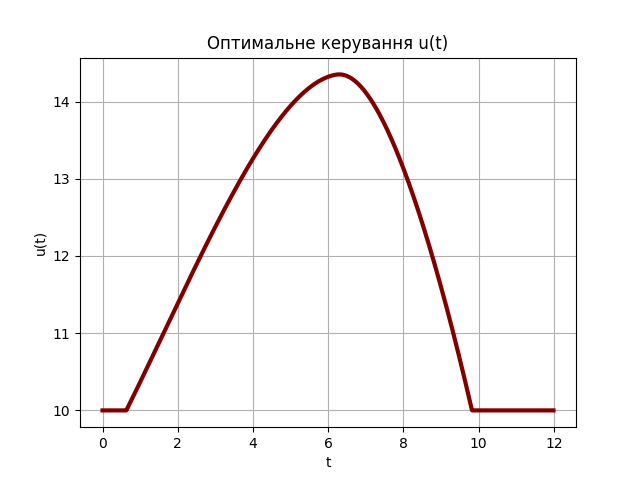
\includegraphics[height=10cm, width=15cm]{figures/stock_management_optimal_control.png} 
\caption{Оптимальне керування в задачі оптимального управління запасами}
\label{im:1.1}
\end{figure}

\begin{figure}[H]
\centering
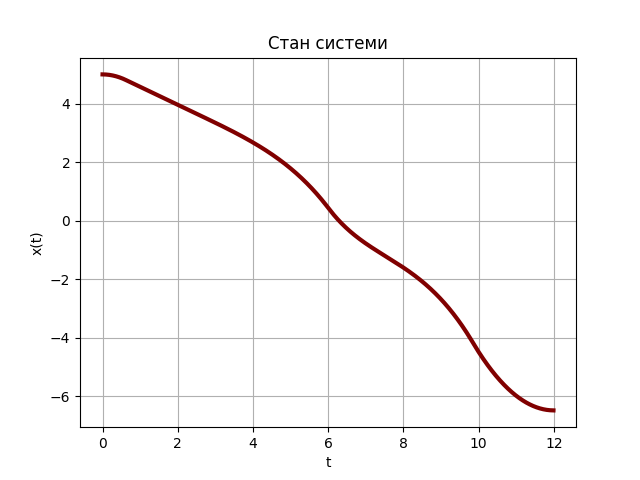
\includegraphics[height=10cm, width=15cm]{figures/State_1d_optimal_stock_management.png}
\caption{Оптимальна траєкторія в задачі оптимального управління запасами}
\label{im:1.2}
\end{figure}

\subsection{Приклад задачі з аналітичним рішенням}
Розглянемо наступну задачу оптимального керування:
$$ \text { Мінімізувати } \frac{1}{2} \int_0^1\left(u^2(t)+x^2(t)\right) d t $$, де
$u \in L^2(0,1)$, $x=x^u$ - оптимальна траєкторія
Рівняння стану має вигляд:
$$
\left\{\begin{array}{l}
    x^{\prime}(t)=u(t), \quad t \in(0,1) \\
    x(0)=1
    \end{array}\right.
$$
Можна встановити, що рівняння спряженого стану має вигляд:
$$
\left\{\begin{array}{l}
    p^{\prime}(t)=-x^u(t), \quad t \in(0,1) \\
    p(1)=0
    \end{array}\right.
$$
Градієнт функції втрат має вигляд:
$$\Phi_u(u)=u+p^u $$
Оптимальне керування задачі:
$$ u^*(t)=-\frac{\sinh (1-t)}{\cosh (1)} $$
Оптимальна траєкторія:
$$
x^*(t)=\frac{\cosh (1-t)}{\cosh (1)}
$$ 
На цьому прикладі можна порівняти аналітичний розвязок та його чисельну апроксимацію методом Арміджіо
\begin{figure}[H]
    \centering
\includegraphics[height=10cm, width=15cm]{figures/States_1d_compare.png} 
\caption{Оптимальна траєкторія в задачі з розділу ???}
\label{im:2.1}
\end{figure}

\begin{figure}[H]
    \centering
\includegraphics[height=10cm, width=15cm]{figures/Control_1d_compare.png}
\caption{Оптимальне керування в задачі в задачі з аналітичним рішенням}
\label{im:2.2}
\end{figure}

\begin{figure}[H]
    \centering
\includegraphics[height=10cm, width=15cm]{figures/Error_control_1d.png}
\caption{Похибка в апроксимації оптимального керування в задачі з аналітичним рішенням}
\label{im:2.3}
\end{figure}

\subsection{Одновимірна задача оптимального збору урожаю}\label{ss_res:2}
\begin{figure}[H]
    \centering
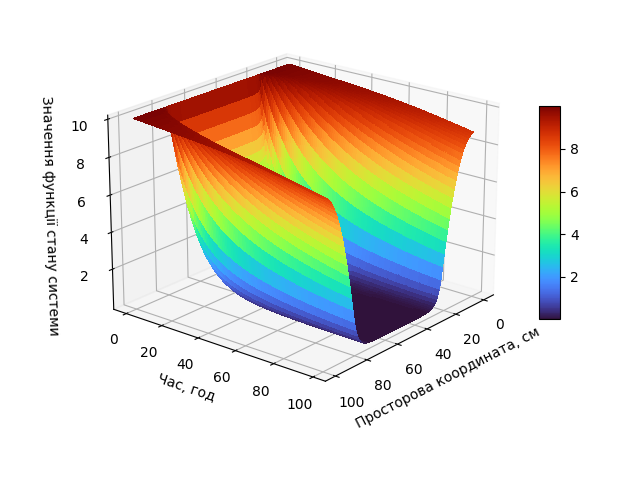
\includegraphics[height=10cm, width=15cm]{figures/State_1d_task_3d_plot.png}
\caption{Оптимальна траєкторія в задачі оптимального збору урожаю}
\label{im:3.1}
\end{figure}

\begin{figure}[H]
\centering
\includegraphics[height=10cm, width=15cm]{figures/Control_1d_3d_harvesting.png}
\caption{Оптимальне керування в задачі оптимального збору урожаю}
\label{im:3.2}
\end{figure}


\subsection{Двовимірна задача оптимального вирощування}\label{ss_res:3}
\begin{figure}[H]
    \centering
\includegraphics[height=10cm, width=15cm]{figures/State_last_2d_harvesting_3d.png}
\caption{Значення оптимальної траєкторії в кінцевий момент часу для двовимірної задачі оптимального збору урожаю}
\label{im:4.1}
\end{figure}

\begin{figure}[H]
\centering
\includegraphics[height=10cm, width=15cm]{figures/State_first_2d_harvesting_3d.png}
\caption{Значення оптимальної траєкторії в початковий момент часу для двовимірної задачі оптимального збору урожаю}
\label{im:4.2}
\end{figure}
\begin{figure}[H]
\centering
\includegraphics[height=10cm, width=15cm]{figures/Control_first_2d_3d_harvesting.png}
\caption{Значення оптимального керування в початковий момент часу для двовимірної задачі оптимального збору урожаю}
\label{im:4.3}
\end{figure}
\begin{figure}[H]
\centering
\includegraphics[height=10cm, width=15cm]{figures/Control_last_harvesting_2d_3d.png}
\caption{Значення оптимального керування в кінцевий момент часу для двовимірної задачі оптимального збору урожаю}
\label{im:4.4}
\end{figure}
\chapter{Висновок} 
У даній роботі розглянуто ряд класичних задач оптимального керування динамічними система з чисельною
реалізацією на мові Python з використанням пакетів з відкритим кодом NumPy та SciPy. Наведені приклади включають моделі 
зі звичайними рівняннями стану, а також рівняннями у частинних похідних. Результати наведені з використанням дво- та трьохвимірних
графіків з пакету Matplotlib. Програманий код реалізовано з використанням парадигми об'єктно-орієнтованого програмування, що
дозволяє перевикористовувати спільні частини алгоритму для різних типів задач. Ієрархія класів побудована таким чином, що 
метод Арміджіо визначено у найстаршому класі-усі класи нащадки визначають поведінку конкретної задачі, що дозволяє витратити
незначні зусилля для розв'язку нових типів задач. 
Розробка програмних пакетів для задач оптимального керування залишається актуальною, оскільки кожна проблема є певною мірою індивідуальна 
і складно піддається узагальненням. 

\newpage
\addcontentsline{toc}{chapter}{Література}
\begin{thebibliography}{9}
\bibitem{1}     https://www.mathworks.com/matlabcentral/fileexchange/25889-an-optimal-control-tutorial-for-beginners
\bibitem{2}   https://www.mathworks.com/matlabcentral/fileexchange/71566-openocl-open-optimal-control-library
\bibitem{3} An Introduction to Optimal Control Problems in Life Sciences and Economics, Sebastian Anita,Viorel Arnautu, Vincenzo Capasso
\bibitem{4} https://digital.library.adelaide.edu.au/dspace/bitstream/2440/15125/1/152.pdf
\end{thebibliography}
 
\chapter*{Додатки}
\addcontentsline{toc}{chapter}{Додатки}
 
\subsection*{Метод Рунге-Кутта}
% Посилання. -   Tan, Delin; Chen, Zheng (2012), ["On A General Formula of Fourth Order Runge-Kutta Method"](http://msme.us/2012-2-1.pdf) (PDF), _Journal of Mathematical Science & Mathematics Education_, **7** (2): 1–10.
    % Алгоритм
    Розглянемо задачу Коші:
    $$
    \left\{\begin{array}{l}
    y^{\prime}(x)=f(x, y(x)) \\
    y\left(x_0\right)=y_0
    \end{array}\right.
    $$
    де $y_0 \in \mathbb{R}$, $f: D \rightarrow \mathbb{R}$, де 
    $$
    D=\left\{(x, y) \in \mathbb{R}^2 ;\left|x-x_0\right| \leq a,\left|y-y_0\right| \leq b\right\} \quad(a, b>0)
    $$
    Тоді розв'язок шукається за наступною рекурентною формулою:
    $$
    \begin{aligned}
    y_{n+1} &=y_n+\frac{1}{6}\left(k_1+2 k_2+2 k_3+k_4\right) h \\
    t_{n+1} &=t_n+h
    \end{aligned}
    $$
    де $h$ - крок дискретизації,
    $$
    \begin{aligned}
    &k_1=f\left(t_n, y_n\right) \\
    &k_2=f\left(t_n+\frac{h}{2}, y_n+h \frac{k_1}{2}\right) \\
    &k_3=f\left(t_n+\frac{h}{2}, y_n+h \frac{k_2}{2}\right) \\
    &k_4=f\left(t_n+h, y_n+h k_3\right) .
    \end{aligned}
    $$
    для усіх $n=0,1,2,3, \ldots, N$, де $N = [T/h], T$  - верхня межа інтегрування по часу.
    \newpage
    Приклад коду мовою Python:
    \begin{python}
import numpy as np  
    
    
def runge_kutta_4order(t_prev, func_value_prev, func, h):  
    k1 = func(t_prev, func_value_prev)  
    k2 = func(t_prev + h/2, func_value_prev + k1*h/2)  
    k3 = func(t_prev + h/2, func_value_prev + k2*h/2)  
    k4 = func(t_prev + h, func_value_prev + k3*h)  
    return func_value_prev + (k1 + 2*k2 + 2*k3 + k4)*h/6  
    
    
def solve_ivp(right_side_function, initial_state, terminate_argument, discrete_param, backward=False):  
    if backward:  
        adjusted_right_side_function = lambda argument, state: -right_side_function(argument, state)  
    else:  
        adjusted_right_side_function = right_side_function  
    states = [initial_state, ]  
    state_prev = states[0]  
    arg_prev = 0  
    arg_space = np.arange(discrete_param, terminate_argument, discrete_param) if not backward else \  
        np.arange(terminate_argument-2*discrete_param, -discrete_param, -discrete_param)  
    
    for arg in arg_space:  
        state_new = runge_kutta_4order(arg_prev, state_prev, 
                        adjusted_right_side_function, 
                        discrete_param)  
        states.append(state_new)  
        arg_prev = arg  
        state_prev = state_new  
    if backward:  
        states = states[::-1]  
    return np.array(states)
        
        \end{python}
        % \end{lstlisting}
        Код оформлено з урахуванням можливості розв'язку зворотного ходу в задачі Коші.
\addcontentsline{toc}{subsection}{Метод Рунге-Кутта}
\newpage
\subsection*{Апроксимація оператора Лапласа для одно- та двовимірної задачі}
Приклад коду мовою Python:
\begin{python}
def laplacian_operator_approximation_2d(state_t, h):
    transformed_state = np.zeros_like(state_t)
    for x_1 in range(transformed_state.shape[0]):
        for x_2 in range(transformed_state.shape[1]):
            left = (state_t[x_1 - 1, x_2] if x_1 != 0 else state_t[x_1, x_2])
            right = (state_t[x_1 + 1, x_2] if x_1 != state_t.shape[0]-1 else state_t[x_1, x_2])
            bottom = (state_t[x_1, x_2 - 1] if x_2 != 0 else state_t[x_1, x_2])
            top = (state_t[x_1, x_2 + 1] if x_2 != state_t.shape[1]-1 else state_t[x_1, x_2])
            current = state_t[x_1, x_2]
            transformed_state[x_1, x_2] = (left + right + bottom + top - 4 * current)/(h ** 2)
    return transformed_state


def laplacian_operator_approximation_1d(state_t, h):
    transformed_state = np.zeros_like(state_t)
    for x_1 in range(transformed_state.shape[0]):
        if x_1 == 0:
            transformed_state[x_1] = (state_t[x_1] + state_t[x_1 + 1] - 2 * state_t[x_1]) / (h ** 2)
        elif x_1 == transformed_state.shape[0] - 1:
            transformed_state[x_1] = (state_t[x_1 - 1] + state_t[x_1] - 2 * state_t[x_1]) / (h ** 2)
        else:
             transformed_state[x_1] = (state_t[x_1 - 1] + state_t[x_1 + 1] - 2 * state_t[x_1]) / (h ** 2)
    return transformed_state
\end{python}
\addcontentsline{toc}{subsection}{Апроксимація оператора Лапласа для одно- та двовимірної задачі}
\newpage
\subsection*{Алгоритм Armijo мовою Python}
Приклад коду мовою Python:
\begin{python}[utf8]
import logging
import numpy as np
import matplotlib.pyplot as plt
    
    
from typing import Callable
from dataclasses import dataclass
from abc import ABC, abstractmethod
    
from src.utils import l2_norm, viz_1d_control, viz_2d_heatmap, viz_2d_time_gif, viz_3d_plot
from src.ode_utils import solve_ivp
    
    
class PMPProjectedGradientSolver(ABC):
        def __init__(self, state_equation_function: Callable, adjoint_state_equation_function: Callable,
                     integrand_cost_function: Callable, cost_derivative_u_function: Callable,
                     projection_gradient_operator: Callable, problem_name: str, init_u: np.array,
                     terminate_time: int, boundary_space: np.array = None, initial_state: np.array=None,
                     eps_cost_derivative: np.float16 = 1e-2, eps_gradient_step: np.float16 = 1e-2,
                     init_gradient_step: np.float16 = 1.0,
                     gradient_adjustment: np.float16 = 0.6,
                     time_grid_step: np.float16 = 1e-2, space_grid_step: np.float16 = None,
                     gradient_step_max_iter: int = 20,
                     ):
    
            self.logger = logging.getLogger('PMPSolver_logger')
            self.logger.setLevel(logging.DEBUG)
            ch = logging.StreamHandler()
            ch.setLevel(logging.INFO)
            formatter = logging.Formatter('%(asctime)s - %(name)s - %(levelname)s - %(message)s')
            ch.setFormatter(formatter)
            self.logger.addHandler(ch)
            self.problem_name = problem_name
            self.logger.info(f'Ініціалізується задача {self.problem_name}')
            self.eps_cost_derivative = eps_cost_derivative
            self.eps_gradient_step = eps_gradient_step
            self.init_gradient_step = init_gradient_step
            self.gradient_adjustment = gradient_adjustment
            self.time_grid_step = time_grid_step
            self.terminate_time = terminate_time
            self.init_u = init_u
            self.boundary_space = boundary_space
            self.init_state = initial_state
    
            self.gradient_step_max_iter = gradient_step_max_iter
            self.logger.info(f'Порядок збіжності градієнта функції втрат: {self.eps_cost_derivative}')
            self.logger.info(f'Порядок збіжності кроку градієнта: {self.eps_gradient_step}')
            self.logger.info(f'Початковий крок градієнта: {self.init_gradient_step}')
            self.logger.info(f'Крок дискретизації по часу: {self.time_grid_step}')
            self.logger.info(f'Кінцеве значення часу: {self.terminate_time}')
            if space_grid_step is not None:
                self.space_grid_step = space_grid_step
                self.logger.info(f'Крок дискретизації по просторовій змінній: {self.space_grid_step}')
            self.logger.info(f'Початковий вектор керування: {self.init_u}')
            self.logger.info(f'Максимальна кількість ітерацій для пошуку найкращого кроку градієнтного спуску: {self.gradient_step_max_iter}')
    
            # Визнчимо функції (оператори) для рівнянь стану та спряженого стану
            self.state_equation_function = state_equation_function
            self.adjoint_state_equation_function = adjoint_state_equation_function
            self.cost_derivative_u_function = cost_derivative_u_function
            self.integrand_cost_function = integrand_cost_function
            self.gradient_projection_function = projection_gradient_operator
    
            # Визначаємо вектори часу та простору
            self.time_range = np.arange(0, self.terminate_time, self.time_grid_step)
    
            # Присвоєння початкових умов
            self.current_gradient_iteration = 0
            self.current_cost_derivative_u = np.array([np.inf])
            self.current_cost = np.inf
            self.new_cost = self.current_cost
            self.current_gradient_step = self.init_gradient_step
            self.current_gradient_step_iteration = 0
            self.current_u = self.init_u
            self.new_u = self.current_u
            if self.init_state is np.ndarray:
                self.space_dimension = self.init_state.shape
            else:
                self.space_dimension = 1
            print(f'Просторова розмірність задачі: {self.space_dimension}')
    
        def norm_gradient_stop_condition(self) -> bool:
            grad_norm = l2_norm(self.current_cost_derivative_u)
            return grad_norm < self.eps_cost_derivative
    
        def gradient_descent_loop_stop_condition(self) -> bool:
            stop_condition = (self.norm_gradient_stop_condition() &
                              (self.current_gradient_step < self.eps_gradient_step))
            return stop_condition
    
        @abstractmethod
        def visualize_control(self, *args, **kwargs) -> None:
            pass
    
        @abstractmethod
        def solve_state_problem(self,  *args, **kwargs) -> np.array:
            pass
    
        @abstractmethod
        def solve_adjoint_state_problem(self, *args, **kwargs) -> np.array:
            pass
    
        @abstractmethod
        def integrate_cost(self, integrand_cost_function) -> np.float32:
            pass
    
        def adjust_gradient_step(self, *args, **kwargs) -> None:
            self.current_gradient_step *= self.gradient_adjustment
    
        def gradient_descent_loop(self) -> None:
    
            # На кожній ітерації перевірка умов збіжності алгоритму
            while not self.gradient_descent_loop_stop_condition():
    
                self.current_cost = self.new_cost
    
                # Розв'язок рівняння стану
                self.current_state = self.solve_state_problem(self.current_u)
                self.logger.info('State')
               # self.logger.info(self.current_state)
                # Розв'язок рівняння спряженого стану
                self.current_adjoint_state = self.solve_adjoint_state_problem(self.current_state, self.current_u)
                self.logger.info('adjoint State')
                #self.logger.info(self.current_adjoint_state)
                # Обчислення градієнита функції втрат з урахуванням аналітичної формули похідної по керуванню
                self.current_cost_derivative_u = self.cost_derivative_u_function(self.current_u, self.current_state,
                                                                                 self.current_adjoint_state)
    
                # Перевірка умови на норму градієнта
                if self.norm_gradient_stop_condition():
                    self.logger.info('Збіжності досягнуто')
                    break
    
                self.logger.info(f'''Значення функції втрат: {self.current_cost}; 
                                    значення l2-норми градієнта: {l2_norm(self.current_cost_derivative_u)};
                                    ітерація №{self.current_gradient_iteration}.''')
                # Пошук кроку градієнтного спуску
                # На кожній ітерації виконується перевірка на величину поточного кроку та на приріст функції втрат
                self.current_gradient_step = self.init_gradient_step
                for i in range(0, self.gradient_step_max_iter):
                    if self.current_gradient_step < self.eps_gradient_step:
                        break
    
                    print('Current u',self.current_u)
                    print('Current gradient step', self.current_gradient_step)
                    print('Current cost derivative', self.current_cost_derivative_u)
                    # Обчислення нового керування
                    self.new_u = self.gradient_projection_function(self.current_u - self.current_gradient_step *
                                                                  self.current_cost_derivative_u)
                    print('cost_derivative')
                    print('New u',self.new_u)
                    # Розв'язок нового рівняння стану
                    self.new_state = self.solve_state_problem(self.new_u)
    
                    # Розв'язок рівняння спряженого стану
                    self.new_adjoint_state = self.solve_adjoint_state_problem(self.new_state, self.new_u)
    
                    # Обчислення нового значення функції втрат
                    cost_func = np.vectorize(self.integrand_cost_function(self.new_state, self.new_adjoint_state, self.new_u))
                    self.new_cost = self.integrate_cost(cost_func)
    
                    #print(self.new_cost)
                    if self.new_cost >= self.current_cost:
                        self.adjust_gradient_step()
                    else:
                        self.current_u = self.new_u
                        break
                else:
                    self.current_u = self.new_u
    
                self.current_gradient_iteration += 1
    
                # Додаткова умова виходу, коли функція втрат збігається
                if np.abs(self.new_cost - self.current_cost) <= self.eps_cost_derivative:
                    self.logger.info(f'Збіжності досягнуто. Значення функціоналу: {-self.current_cost}')
                    if self.space_dimension == 2:
                        viz_2d_time_gif([self.current_state[slice_idx, :, :] for slice_idx in range(self.current_state.shape[0])],
                                        'Оптипмальний контроль вирощування, 2 виміри')
                        viz_2d_time_gif(
                            [self.current_state[slice_idx, :, :] for slice_idx in range(self.current_state.shape[0])],
                            'Стан при оптмальному керуванні, 2 виміри')
                    break
            else:
                self.logger.info(f'Збіжності досягнуто. Значення функціоналу: {-self.current_cost}')
                if self.space_dimension == 2:
                    viz_2d_time_gif([self.current_state[slice_idx, :, :] for slice_idx in range(self.current_state.shape[0])],
                                    'Оптипмальний контроль вирощування, 2 виміри')
                    viz_2d_time_gif(
                        [self.current_state[slice_idx, :, :] for slice_idx in range(self.current_state.shape[0])],
                        'Стан при оптмальному керуванні, 2 виміри')
    
    
class PMPODESolver(PMPProjectedGradientSolver):
        def __init__(self, state_equation_function: Callable, adjoint_state_equation_function: Callable,
                     integrand_cost_function: Callable, cost_derivative_u_function: Callable,
                     projection_gradient_operator: Callable, problem_name: str, init_u: np.array,
                     terminate_time: int, boundary_space: np.array = None, initial_state: np.array=None,
                     eps_cost_derivative: np.float16 = 1e-3, eps_gradient_step: np.float16 = 1e-3,
                     init_gradient_step: np.float16 = 1.0, gradient_adjustment: np.float16 = 0.6,
                     time_grid_step: np.float16 = 1e-2, space_grid_step: np.float16 = None,
                     gradient_step_max_iter: int = 20):
    
            super().__init__(state_equation_function, adjoint_state_equation_function,
                     integrand_cost_function, cost_derivative_u_function,
                     projection_gradient_operator, problem_name, init_u,
                     terminate_time, boundary_space, initial_state,
                     eps_cost_derivative, eps_gradient_step,
                     init_gradient_step,gradient_adjustment,
                     time_grid_step, space_grid_step,
                     gradient_step_max_iter)
    
        def visualize_control(self):
            viz_1d_control(self.time_range, self.current_u, "Оптимальне керування u(t)", "t", "u(t)")
            viz_1d_control(self.time_range, self.current_state, "Стан системи", "t", "x(t)")
    
        def solve_state_problem(self, u) -> np.array:
            state = solve_ivp(self.state_equation_function(u), self.init_state, self.terminate_time, self.time_grid_step)
            return state
    
        def solve_adjoint_state_problem(self, state, u) -> np.array:
            adjoint_state = solve_ivp(self.adjoint_state_equation_function(state, u), 0.0,
                                      self.terminate_time, self.time_grid_step, backward=True)
            return adjoint_state
    
        def integrate_cost(self, integrand_cost_function: Callable):
            return np.trapz(y=integrand_cost_function(self.time_range), x=self.time_range, dx=self.time_grid_step)
    
    
class PMPPDESolver(PMPProjectedGradientSolver):
        def __init__(self, *args, **kwargs):
            super().__init__(*args, **kwargs)
    
        def visualize_control(self, dimensions: int = 2) -> None:
    
            if dimensions == 2:
                print(self.current_u)
                viz_2d_heatmap(self.current_u, 'Оптимальний контроль', save=True)
                viz_2d_heatmap(self.current_state, 'Стан системи', save=True)
                viz_2d_heatmap(self.current_state, 'Стан системи', save=True)
    
                viz_3d_plot(self.current_u, 'Оптимальний контроль', save=True)
                viz_3d_plot(self.current_state, 'Оптимальний контроль', save=True)
            elif dimensions == 3:
                print(self.current_u)
                print(self.current_u.shape)
                viz_2d_heatmap(self.current_u[0, :, :], 'Оптимальний контроль на початку', save=True)
                viz_2d_heatmap(self.current_state[0, :, :], 'Системи на початку', save=True)
                viz_2d_heatmap(self.current_u[-1, :, :], 'Оптимальний контроль в кінці', save=True)
                viz_2d_heatmap(self.current_state[-1, :, :], 'Системи в кінці', save=True)
                viz_3d_plot(self.current_state[-1, :, :], 'Система в останній момент часу', save=True)
                viz_3d_plot(self.current_state[0, :, :], 'Системи в початковий момент часу', save=True)
                viz_3d_plot(self.current_u[-1, :, :], 'Оптимальне керування в останній момент часу', save=True)
                viz_3d_plot(self.current_u[0, :, :], 'Оптимальне керування в початковий момент часу', save=True)
    
            else:
                viz_1d_control(self.time_range, self.current_u)
    
        def solve_state_problem(self, u) -> np.array:
            state = solve_ivp(self.state_equation_function(u), self.init_state, self.terminate_time, self.time_grid_step)
            return state
    
        def solve_adjoint_state_problem(self, state, u) -> np.array:
            adjoint_state = solve_ivp(self.adjoint_state_equation_function(state, u), np.zeros_like(self.init_state),
                                      self.terminate_time, self.time_grid_step, backward=True)
            return adjoint_state
    
        def integrate_cost(self, integrand_cost_function: Callable):
            return np.trapz(y=integrand_cost_function(self.time_range), x=self.time_range, dx=self.time_grid_step)
    
    
\end{python}
\addcontentsline{toc}{subsection}{Апроксимація оператора Лапласа для одно- та двовимірної задачі}
\end{document}